% Options for packages loaded elsewhere
\PassOptionsToPackage{unicode}{hyperref}
\PassOptionsToPackage{hyphens}{url}
%
\documentclass[
]{book}
\usepackage{lmodern}
\usepackage{amssymb,amsmath}
\usepackage{ifxetex,ifluatex}
\ifnum 0\ifxetex 1\fi\ifluatex 1\fi=0 % if pdftex
  \usepackage[T1]{fontenc}
  \usepackage[utf8]{inputenc}
  \usepackage{textcomp} % provide euro and other symbols
\else % if luatex or xetex
  \usepackage{unicode-math}
  \defaultfontfeatures{Scale=MatchLowercase}
  \defaultfontfeatures[\rmfamily]{Ligatures=TeX,Scale=1}
\fi
% Use upquote if available, for straight quotes in verbatim environments
\IfFileExists{upquote.sty}{\usepackage{upquote}}{}
\IfFileExists{microtype.sty}{% use microtype if available
  \usepackage[]{microtype}
  \UseMicrotypeSet[protrusion]{basicmath} % disable protrusion for tt fonts
}{}
\makeatletter
\@ifundefined{KOMAClassName}{% if non-KOMA class
  \IfFileExists{parskip.sty}{%
    \usepackage{parskip}
  }{% else
    \setlength{\parindent}{0pt}
    \setlength{\parskip}{6pt plus 2pt minus 1pt}}
}{% if KOMA class
  \KOMAoptions{parskip=half}}
\makeatother
\usepackage{xcolor}
\IfFileExists{xurl.sty}{\usepackage{xurl}}{} % add URL line breaks if available
\IfFileExists{bookmark.sty}{\usepackage{bookmark}}{\usepackage{hyperref}}
\hypersetup{
  pdftitle={Python医療データ分析本をRでやる},
  pdfauthor={gg\_hatano},
  hidelinks,
  pdfcreator={LaTeX via pandoc}}
\urlstyle{same} % disable monospaced font for URLs
\usepackage{color}
\usepackage{fancyvrb}
\newcommand{\VerbBar}{|}
\newcommand{\VERB}{\Verb[commandchars=\\\{\}]}
\DefineVerbatimEnvironment{Highlighting}{Verbatim}{commandchars=\\\{\}}
% Add ',fontsize=\small' for more characters per line
\usepackage{framed}
\definecolor{shadecolor}{RGB}{248,248,248}
\newenvironment{Shaded}{\begin{snugshade}}{\end{snugshade}}
\newcommand{\AlertTok}[1]{\textcolor[rgb]{0.94,0.16,0.16}{#1}}
\newcommand{\AnnotationTok}[1]{\textcolor[rgb]{0.56,0.35,0.01}{\textbf{\textit{#1}}}}
\newcommand{\AttributeTok}[1]{\textcolor[rgb]{0.77,0.63,0.00}{#1}}
\newcommand{\BaseNTok}[1]{\textcolor[rgb]{0.00,0.00,0.81}{#1}}
\newcommand{\BuiltInTok}[1]{#1}
\newcommand{\CharTok}[1]{\textcolor[rgb]{0.31,0.60,0.02}{#1}}
\newcommand{\CommentTok}[1]{\textcolor[rgb]{0.56,0.35,0.01}{\textit{#1}}}
\newcommand{\CommentVarTok}[1]{\textcolor[rgb]{0.56,0.35,0.01}{\textbf{\textit{#1}}}}
\newcommand{\ConstantTok}[1]{\textcolor[rgb]{0.00,0.00,0.00}{#1}}
\newcommand{\ControlFlowTok}[1]{\textcolor[rgb]{0.13,0.29,0.53}{\textbf{#1}}}
\newcommand{\DataTypeTok}[1]{\textcolor[rgb]{0.13,0.29,0.53}{#1}}
\newcommand{\DecValTok}[1]{\textcolor[rgb]{0.00,0.00,0.81}{#1}}
\newcommand{\DocumentationTok}[1]{\textcolor[rgb]{0.56,0.35,0.01}{\textbf{\textit{#1}}}}
\newcommand{\ErrorTok}[1]{\textcolor[rgb]{0.64,0.00,0.00}{\textbf{#1}}}
\newcommand{\ExtensionTok}[1]{#1}
\newcommand{\FloatTok}[1]{\textcolor[rgb]{0.00,0.00,0.81}{#1}}
\newcommand{\FunctionTok}[1]{\textcolor[rgb]{0.00,0.00,0.00}{#1}}
\newcommand{\ImportTok}[1]{#1}
\newcommand{\InformationTok}[1]{\textcolor[rgb]{0.56,0.35,0.01}{\textbf{\textit{#1}}}}
\newcommand{\KeywordTok}[1]{\textcolor[rgb]{0.13,0.29,0.53}{\textbf{#1}}}
\newcommand{\NormalTok}[1]{#1}
\newcommand{\OperatorTok}[1]{\textcolor[rgb]{0.81,0.36,0.00}{\textbf{#1}}}
\newcommand{\OtherTok}[1]{\textcolor[rgb]{0.56,0.35,0.01}{#1}}
\newcommand{\PreprocessorTok}[1]{\textcolor[rgb]{0.56,0.35,0.01}{\textit{#1}}}
\newcommand{\RegionMarkerTok}[1]{#1}
\newcommand{\SpecialCharTok}[1]{\textcolor[rgb]{0.00,0.00,0.00}{#1}}
\newcommand{\SpecialStringTok}[1]{\textcolor[rgb]{0.31,0.60,0.02}{#1}}
\newcommand{\StringTok}[1]{\textcolor[rgb]{0.31,0.60,0.02}{#1}}
\newcommand{\VariableTok}[1]{\textcolor[rgb]{0.00,0.00,0.00}{#1}}
\newcommand{\VerbatimStringTok}[1]{\textcolor[rgb]{0.31,0.60,0.02}{#1}}
\newcommand{\WarningTok}[1]{\textcolor[rgb]{0.56,0.35,0.01}{\textbf{\textit{#1}}}}
\usepackage{longtable,booktabs}
% Correct order of tables after \paragraph or \subparagraph
\usepackage{etoolbox}
\makeatletter
\patchcmd\longtable{\par}{\if@noskipsec\mbox{}\fi\par}{}{}
\makeatother
% Allow footnotes in longtable head/foot
\IfFileExists{footnotehyper.sty}{\usepackage{footnotehyper}}{\usepackage{footnote}}
\makesavenoteenv{longtable}
\usepackage{graphicx,grffile}
\makeatletter
\def\maxwidth{\ifdim\Gin@nat@width>\linewidth\linewidth\else\Gin@nat@width\fi}
\def\maxheight{\ifdim\Gin@nat@height>\textheight\textheight\else\Gin@nat@height\fi}
\makeatother
% Scale images if necessary, so that they will not overflow the page
% margins by default, and it is still possible to overwrite the defaults
% using explicit options in \includegraphics[width, height, ...]{}
\setkeys{Gin}{width=\maxwidth,height=\maxheight,keepaspectratio}
% Set default figure placement to htbp
\makeatletter
\def\fps@figure{htbp}
\makeatother
\setlength{\emergencystretch}{3em} % prevent overfull lines
\providecommand{\tightlist}{%
  \setlength{\itemsep}{0pt}\setlength{\parskip}{0pt}}
\setcounter{secnumdepth}{5}
\usepackage{booktabs}
\usepackage[]{natbib}
\bibliographystyle{apalike}

\title{Python医療データ分析本をRでやる}
\author{gg\_hatano}
\date{2020-08-24}

\begin{document}
\maketitle

{
\setcounter{tocdepth}{1}
\tableofcontents
}
\hypertarget{ux306fux3058ux3081ux306b}{%
\chapter{はじめに}\label{ux306fux3058ux3081ux306b}}

\hypertarget{ux3053ux306eux672cux3067ux3084ux308bux3053ux3068}{%
\section{この本でやること}\label{ux3053ux306eux672cux3067ux3084ux308bux3053ux3068}}

\href{https://gihyo.jp/book/2020/978-4-297-11517-3}{Pythonによる医療データ分析入門―pandas+擬似レセプト編}をRでやってみる、という内容です。

ソースコードは\href{https://github.com/gghatano/python_synthetic_medical_data}{GitHub}にも置いていきます。

\hypertarget{ux6ce8ux610fux70b9}{%
\section{注意点}\label{ux6ce8ux610fux70b9}}

Rでやるので、参考文献と比べて実装方針が異なるところはあると思います。

\hypertarget{ux6b7bux4ea1ux7387ux306eux63a8ux5b9a}{%
\chapter{死亡率の推定}\label{ux6b7bux4ea1ux7387ux306eux63a8ux5b9a}}

1章です。

\hypertarget{ux65e5ux672cux7248ux6b7bux4ea1ux30c7ux30fcux30bfux30d9ux30fcux30b9ux306eux5229ux7528}{%
\section{「日本版死亡データベース」の利用}\label{ux65e5ux672cux7248ux6b7bux4ea1ux30c7ux30fcux30bfux30d9ux30fcux30b9ux306eux5229ux7528}}

健保組合データを擬似生成するために、出生・志望の公的統計を利用して、乱数でシミュレーションする。

\hypertarget{ux51faux751fux7387ux30c7ux30fcux30bfux306eux53d6ux5f97}{%
\subsection{出生率データの取得}\label{ux51faux751fux7387ux30c7ux30fcux30bfux306eux53d6ux5f97}}

\href{http://www.ipss.go.jp/}{IPSS}が公開している、年次出生数のデータを利用する。

\begin{Shaded}
\begin{Highlighting}[]
\KeywordTok{library}\NormalTok{(readr)}
\KeywordTok{library}\NormalTok{(dplyr)}
\NormalTok{url =}\StringTok{ 'http://www.ipss.go.jp/p-toukei/JMD/00/STATS/Births.txt'}
\NormalTok{dat =}\StringTok{ }\KeywordTok{read.table}\NormalTok{(url, }\DataTypeTok{skip=}\DecValTok{2}\NormalTok{, }\DataTypeTok{header =} \OtherTok{TRUE}\NormalTok{)}
\NormalTok{dat }\OperatorTok\StringTok{ }\NormalTok{head}
\end{Highlighting}
\end{Shaded}

\begin{verbatim}
##   Year  Female    Male   Total
## 1 1947 1301806 1376986 2678792
## 2 1948 1303060 1378564 2681624
## 3 1949 1316630 1380008 2696638
## 4 1950 1134396 1203111 2337507
## 5 1951 1043048 1094641 2137689
## 6 1952  977101 1028061 2005162
\end{verbatim}

ある年に、FemaleとMaleが何人生まれたかのデータになっている。

性別列を作って縦に持っておく。

\begin{Shaded}
\begin{Highlighting}[]
\KeywordTok{library}\NormalTok{(tidyr)}
\KeywordTok{library}\NormalTok{(magrittr)}
\NormalTok{dat }\OperatorTok\StringTok{  }
\StringTok{        }\KeywordTok{pivot_longer}\NormalTok{(}\DataTypeTok{cols =} \KeywordTok{c}\NormalTok{(}\StringTok{"Male"}\NormalTok{, }\StringTok{"Female"}\NormalTok{), }\DataTypeTok{names_to =} \StringTok{"Sex"}\NormalTok{, }\DataTypeTok{values_to =} \StringTok{"Life"}\NormalTok{) }\OperatorTok\StringTok{ }
\StringTok{        }\KeywordTok{mutate}\NormalTok{(}\DataTypeTok{Sex =} \KeywordTok{if_else}\NormalTok{(Sex }\OperatorTok{==}\StringTok{ "Female"}\NormalTok{, }\StringTok{"F"}\NormalTok{, }\StringTok{"M"}\NormalTok{)) ->}\StringTok{ }\NormalTok{dat}
\NormalTok{dat}
\end{Highlighting}
\end{Shaded}

\begin{verbatim}
## # A tibble: 140 x 4
##     Year   Total Sex      Life
##    <int>   <int> <chr>   <int>
##  1  1947 2678792 M     1376986
##  2  1947 2678792 F     1301806
##  3  1948 2681624 M     1378564
##  4  1948 2681624 F     1303060
##  5  1949 2696638 M     1380008
##  6  1949 2696638 F     1316630
##  7  1950 2337507 M     1203111
##  8  1950 2337507 F     1134396
##  9  1951 2137689 M     1094641
## 10  1951 2137689 F     1043048
## # ... with 130 more rows
\end{verbatim}

乱数でシミュレーションをするために、累積比率を出しておく

\begin{Shaded}
\begin{Highlighting}[]
\NormalTok{dat }\OperatorTok
\StringTok{        }\KeywordTok{arrange}\NormalTok{(Sex, Year)}
\NormalTok{dat }\OperatorTok
\StringTok{        }\KeywordTok{mutate}\NormalTok{(}\DataTypeTok{ratio =}\NormalTok{ Life }\OperatorTok{/}\StringTok{ }\KeywordTok{sum}\NormalTok{(Life)) }\OperatorTok
\StringTok{        }\KeywordTok{mutate}\NormalTok{(}\DataTypeTok{cum_sum =} \KeywordTok{cumsum}\NormalTok{(ratio))}

\NormalTok{dat }\OperatorTok\StringTok{ }\NormalTok{head}
\end{Highlighting}
\end{Shaded}

\begin{verbatim}
## # A tibble: 6 x 6
##    Year   Total Sex      Life   ratio cum_sum
##   <int>   <int> <chr>   <int>   <dbl>   <dbl>
## 1  1947 2678792 F     1301806 0.0121   0.0121
## 2  1948 2681624 F     1303060 0.0122   0.0243
## 3  1949 2696638 F     1316630 0.0123   0.0366
## 4  1950 2337507 F     1134396 0.0106   0.0472
## 5  1951 2137689 F     1043048 0.00973  0.0569
## 6  1952 2005162 F      977101 0.00912  0.0660
\end{verbatim}

\begin{Shaded}
\begin{Highlighting}[]
\NormalTok{dat }\OperatorTok\StringTok{ }
\StringTok{        }\KeywordTok{select}\NormalTok{(}\OperatorTok{-}\NormalTok{Total) }\OperatorTok\StringTok{ }
\StringTok{        }\KeywordTok{write.csv}\NormalTok{(}\StringTok{"./data/ipss_birth.csv"}\NormalTok{, }\DataTypeTok{row.names=}\OtherTok{FALSE}\NormalTok{, }\DataTypeTok{quote =} \OtherTok{FALSE}\NormalTok{)}
\end{Highlighting}
\end{Shaded}

累積確率分布を作る。これにより、一様乱数(y軸:0-1)から、対応する行番号が得られて、
行番号から、(出生年,性別)を得ることができる。

欲しい人数分だけ一様乱数を取れば、出生のデータが得られる。

\begin{Shaded}
\begin{Highlighting}[]
\KeywordTok{library}\NormalTok{(ggplot2)}
\NormalTok{dat =}\StringTok{ }\KeywordTok{read_csv}\NormalTok{(}\StringTok{"./data/ipss_birth.csv"}\NormalTok{)}
\end{Highlighting}
\end{Shaded}

\begin{verbatim}
## Parsed with column specification:
## cols(
##   Year = col_double(),
##   Sex = col_character(),
##   Life = col_double(),
##   ratio = col_double(),
##   cum_sum = col_double()
## )
\end{verbatim}

\begin{Shaded}
\begin{Highlighting}[]
\NormalTok{dat }\OperatorTok\StringTok{ }
\StringTok{        }\KeywordTok{mutate}\NormalTok{(}\DataTypeTok{x_axis =} \KeywordTok{paste}\NormalTok{(Year, Sex, }\DataTypeTok{sep=}\StringTok{""}\NormalTok{)) }\OperatorTok\StringTok{ }
\StringTok{        }\KeywordTok{mutate}\NormalTok{(}\DataTypeTok{row_num =} \DecValTok{1}\OperatorTok{:}\KeywordTok{nrow}\NormalTok{(.)) }\OperatorTok\StringTok{ }
\StringTok{        }\KeywordTok{ggplot}\NormalTok{() }\OperatorTok{+}\StringTok{ }
\StringTok{        }\KeywordTok{geom_line}\NormalTok{(}\KeywordTok{aes}\NormalTok{(}\DataTypeTok{x =}\NormalTok{ row_num, }\DataTypeTok{y =}\NormalTok{ cum_sum), }\DataTypeTok{stat =} \StringTok{"identity"}\NormalTok{) }\OperatorTok{+}
\StringTok{        }\KeywordTok{annotate}\NormalTok{(}\StringTok{"segment"}\NormalTok{,}\DataTypeTok{x=}\DecValTok{1}\NormalTok{,}\DataTypeTok{xend=}\DecValTok{90}\NormalTok{,}\DataTypeTok{y=}\FloatTok{0.7}\NormalTok{,}\DataTypeTok{yend=}\FloatTok{0.7}\NormalTok{,}\DataTypeTok{colour=}\StringTok{"blue"}\NormalTok{,}
             \DataTypeTok{size=}\DecValTok{1}\NormalTok{, }\DataTypeTok{arrow=}\KeywordTok{arrow}\NormalTok{()) }\OperatorTok{+}\StringTok{ }
\StringTok{        }\KeywordTok{annotate}\NormalTok{(}\StringTok{"segment"}\NormalTok{,}\DataTypeTok{x=}\DecValTok{92}\NormalTok{,}\DataTypeTok{xend=}\DecValTok{92}\NormalTok{,}\DataTypeTok{y=}\FloatTok{0.65}\NormalTok{,}\DataTypeTok{yend=}\FloatTok{0.0}\NormalTok{,}\DataTypeTok{colour=}\StringTok{"blue"}\NormalTok{,}
                    \DataTypeTok{size=}\DecValTok{1}\NormalTok{,}\DataTypeTok{arrow=}\KeywordTok{arrow}\NormalTok{()) }\OperatorTok{+}\StringTok{ }
\StringTok{        }\KeywordTok{annotate}\NormalTok{(}\StringTok{"text"}\NormalTok{, }\DataTypeTok{x=}\DecValTok{20}\NormalTok{, }\DataTypeTok{y=}\FloatTok{0.75}\NormalTok{, }\DataTypeTok{parse=}\OtherTok{TRUE}\NormalTok{, }\DataTypeTok{label=}\StringTok{"'Random Number 0.7'"}\NormalTok{) }\OperatorTok{+}
\StringTok{        }\KeywordTok{annotate}\NormalTok{(}\StringTok{"text"}\NormalTok{, }\DataTypeTok{x=}\DecValTok{120}\NormalTok{, }\DataTypeTok{y=}\FloatTok{0.2}\NormalTok{, }\DataTypeTok{parse=}\OtherTok{TRUE}\NormalTok{, }\DataTypeTok{label=}\StringTok{"'Rownum: 95 -> 1969-Female'"}\NormalTok{) }\OperatorTok{+}
\StringTok{        }\KeywordTok{ggtitle}\NormalTok{(}\StringTok{"Cumulative ratio of Population Birth"}\NormalTok{)}
\end{Highlighting}
\end{Shaded}

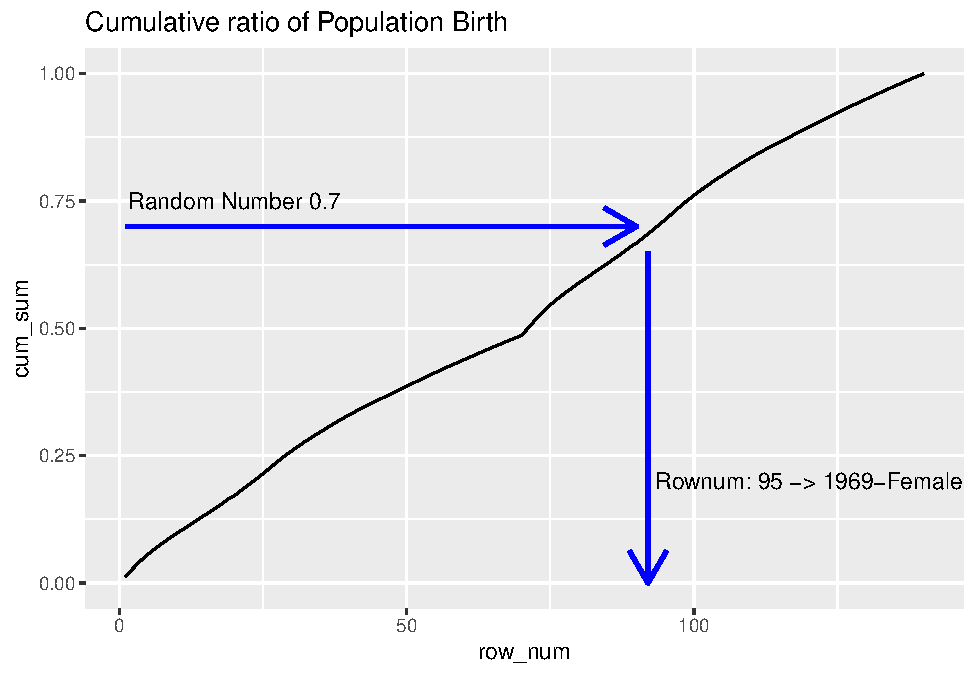
\includegraphics{python-medical-data_files/figure-latex/unnamed-chunk-4-1.pdf}

これを利用して、出生のシミュレーションができる。

\hypertarget{ux6b7bux4ea1ux30c7ux30fcux30bfux306eux53d6ux5f97ux3068ux6574ux5f62}{%
\subsection{死亡データの取得と整形}\label{ux6b7bux4ea1ux30c7ux30fcux30bfux306eux53d6ux5f97ux3068ux6574ux5f62}}

次は、死亡率を算出して、死亡のシミュレーションを行う。

\begin{Shaded}
\begin{Highlighting}[]
\NormalTok{url_death_rate =}\StringTok{ "http://www.ipss.go.jp/p-toukei/JMD/00/STATS/Mx_1x1.txt"}
\NormalTok{dat =}\StringTok{ }\KeywordTok{read.table}\NormalTok{(url_death_rate, }\DataTypeTok{skip=}\DecValTok{2}\NormalTok{, }\DataTypeTok{header =} \OtherTok{TRUE}\NormalTok{)}
\NormalTok{dat }\OperatorTok\StringTok{ }\NormalTok{str}
\end{Highlighting}
\end{Shaded}

\begin{verbatim}
## 'data.frame':	7770 obs. of  5 variables:
##  $ Year  : int  1947 1947 1947 1947 1947 1947 1947 1947 1947 1947 ...
##  $ Age   : chr  "0" "1" "2" "3" ...
##  $ Female: chr  "0.087401" "0.033723" "0.016994" "0.011412" ...
##  $ Male  : chr  "0.099181" "0.034697" "0.016804" "0.011461" ...
##  $ Total : chr  "0.093432" "0.034220" "0.016897" "0.011437" ...
\end{verbatim}

死亡率のデータは、Year年にX才だった人が1年後に死んでいる確率を表している。(本当に?)

今回は簡単のために、2016年の死亡率でシミュレーションを行う。

\begin{Shaded}
\begin{Highlighting}[]
\NormalTok{dat }\OperatorTok\StringTok{ }
\StringTok{        }\KeywordTok{filter}\NormalTok{(Year }\OperatorTok{==}\StringTok{ }\DecValTok{2016}\NormalTok{) }\OperatorTok\StringTok{ }
\StringTok{        }\KeywordTok{select}\NormalTok{(}\OperatorTok{-}\NormalTok{Year) }\OperatorTok\StringTok{ }
\StringTok{        }\KeywordTok{select}\NormalTok{(}\OperatorTok{-}\NormalTok{Total)}
\end{Highlighting}
\end{Shaded}

Ageがcharになっているので、確認する。

\begin{Shaded}
\begin{Highlighting}[]
\NormalTok{dat}\OperatorTok{$}\NormalTok{Age }\OperatorTok\StringTok{ }\NormalTok{table}
\end{Highlighting}
\end{Shaded}

\begin{verbatim}
## .
##    0    1   10  100  101  102  103  104  105  106  107  108  109   11 110+   12 
##    1    1    1    1    1    1    1    1    1    1    1    1    1    1    1    1 
##   13   14   15   16   17   18   19    2   20   21   22   23   24   25   26   27 
##    1    1    1    1    1    1    1    1    1    1    1    1    1    1    1    1 
##   28   29    3   30   31   32   33   34   35   36   37   38   39    4   40   41 
##    1    1    1    1    1    1    1    1    1    1    1    1    1    1    1    1 
##   42   43   44   45   46   47   48   49    5   50   51   52   53   54   55   56 
##    1    1    1    1    1    1    1    1    1    1    1    1    1    1    1    1 
##   57   58   59    6   60   61   62   63   64   65   66   67   68   69    7   70 
##    1    1    1    1    1    1    1    1    1    1    1    1    1    1    1    1 
##   71   72   73   74   75   76   77   78   79    8   80   81   82   83   84   85 
##    1    1    1    1    1    1    1    1    1    1    1    1    1    1    1    1 
##   86   87   88   89    9   90   91   92   93   94   95   96   97   98   99 
##    1    1    1    1    1    1    1    1    1    1    1    1    1    1    1
\end{verbatim}

110+があるので、これは簡単のために111才にしておく。

\begin{Shaded}
\begin{Highlighting}[]
\NormalTok{dat }\OperatorTok
\StringTok{        }\KeywordTok{mutate}\NormalTok{(}\DataTypeTok{Age =} \KeywordTok{if_else}\NormalTok{(Age }\OperatorTok{==}\StringTok{ "110+"}\NormalTok{, }\StringTok{"111"}\NormalTok{, Age)) }\OperatorTok\StringTok{ }
\StringTok{        }\KeywordTok{mutate}\NormalTok{(}\DataTypeTok{Age =} \KeywordTok{as.integer}\NormalTok{(Age)) }

\NormalTok{dat }\OperatorTok
\StringTok{        }\KeywordTok{mutate}\NormalTok{(}\DataTypeTok{Anb =}\NormalTok{ Age) }\OperatorTok\StringTok{ }
\StringTok{        }\KeywordTok{select}\NormalTok{(}\OperatorTok{-}\NormalTok{Age)}

\NormalTok{dat }\OperatorTok\StringTok{ }\NormalTok{head}
\end{Highlighting}
\end{Shaded}

\begin{verbatim}
##     Female     Male Anb
## 1 0.002028 0.001995   0
## 2 0.000313 0.000340   1
## 3 0.000174 0.000178   2
## 4 0.000098 0.000133   3
## 5 0.000087 0.000095   4
## 6 0.000084 0.000101   5
\end{verbatim}

AnbとAlbについては、あとで追記する。Anbなので、Albに直す。

\(x\)才のAnb死亡率\(q_x\)とすると、Alb死亡率は、\(\frac{q_x+q_{x+1}}{2}\)になる。

\begin{Shaded}
\begin{Highlighting}[]
\NormalTok{dat }\OperatorTok
\StringTok{        }\KeywordTok{mutate}\NormalTok{(}\DataTypeTok{Female =} \KeywordTok{as.numeric}\NormalTok{(Female)) }\OperatorTok
\StringTok{        }\KeywordTok{mutate}\NormalTok{(}\DataTypeTok{Male =} \KeywordTok{as.numeric}\NormalTok{(Male)) }\OperatorTok\StringTok{ }
\StringTok{        }\KeywordTok{mutate}\NormalTok{(}\DataTypeTok{lead_Female =} \KeywordTok{lead}\NormalTok{(Female)) }\OperatorTok\StringTok{ }
\StringTok{        }\KeywordTok{mutate}\NormalTok{(}\DataTypeTok{lead_Male =} \KeywordTok{lead}\NormalTok{(Male)) }\OperatorTok\StringTok{ }
\StringTok{        }\KeywordTok{mutate}\NormalTok{(}\DataTypeTok{F =}\NormalTok{ (Female }\OperatorTok{+}\StringTok{ }\NormalTok{lead_Female)}\OperatorTok{/}\DecValTok{2}\NormalTok{) }\OperatorTok\StringTok{ }
\StringTok{        }\KeywordTok{mutate}\NormalTok{(}\DataTypeTok{M =}\NormalTok{ (Male }\OperatorTok{+}\StringTok{ }\NormalTok{lead_Male)}\OperatorTok{/}\DecValTok{2}\NormalTok{) }\OperatorTok\StringTok{ }
\StringTok{        }\KeywordTok{mutate}\NormalTok{(}\DataTypeTok{Alb =}\NormalTok{ Anb) }\OperatorTok\StringTok{ }
\StringTok{        }\KeywordTok{select}\NormalTok{(Alb,F,M)}

\NormalTok{dat }\OperatorTok\StringTok{ }\NormalTok{head}
\end{Highlighting}
\end{Shaded}

\begin{verbatim}
##   Alb         F         M
## 1   0 0.0011705 0.0011675
## 2   1 0.0002435 0.0002590
## 3   2 0.0001360 0.0001555
## 4   3 0.0000925 0.0001140
## 5   4 0.0000855 0.0000980
## 6   5 0.0000815 0.0001060
\end{verbatim}

年次死亡率を可視化してみる。
横軸が年齢、縦軸が1年以内に死亡する確率。

\begin{Shaded}
\begin{Highlighting}[]
\NormalTok{dat }\OperatorTok\StringTok{ }
\StringTok{        }\KeywordTok{pivot_longer}\NormalTok{(}\DataTypeTok{cols=}\KeywordTok{c}\NormalTok{(}\StringTok{"F"}\NormalTok{,}\StringTok{"M"}\NormalTok{), }\DataTypeTok{names_to =} \StringTok{"Sex"}\NormalTok{, }\DataTypeTok{values_to =} \StringTok{"Mortarity"}\NormalTok{) }\OperatorTok\StringTok{ }
\StringTok{        }\KeywordTok{ggplot}\NormalTok{(}\KeywordTok{aes}\NormalTok{(}\DataTypeTok{x =}\NormalTok{ Alb, }\DataTypeTok{y =}\NormalTok{ Mortarity, }\DataTypeTok{group =}\NormalTok{ Sex, }\DataTypeTok{color =}\NormalTok{ Sex)) }\OperatorTok{+}\StringTok{ }
\StringTok{        }\KeywordTok{geom_line}\NormalTok{() }\OperatorTok{+}\StringTok{ }
\StringTok{        }\KeywordTok{geom_hline}\NormalTok{(}\DataTypeTok{yintercept =} \FloatTok{1.0}\NormalTok{, }\DataTypeTok{linetype =} \StringTok{"dashed"}\NormalTok{) }\OperatorTok{+}\StringTok{ }
\StringTok{        }\KeywordTok{annotate}\NormalTok{(}\StringTok{"text"}\NormalTok{, }\DataTypeTok{x =} \DecValTok{10}\NormalTok{, }\DataTypeTok{y =} \FloatTok{1.05}\NormalTok{, }\DataTypeTok{label =} \StringTok{'Mortarity: 1.0'}\NormalTok{) }\OperatorTok{+}\StringTok{ }
\StringTok{        }\KeywordTok{ggtitle}\NormalTok{(}\StringTok{"Mortarity"}\NormalTok{)}
\end{Highlighting}
\end{Shaded}

\begin{verbatim}
## Warning: Removed 2 row(s) containing missing values (geom_path).
\end{verbatim}

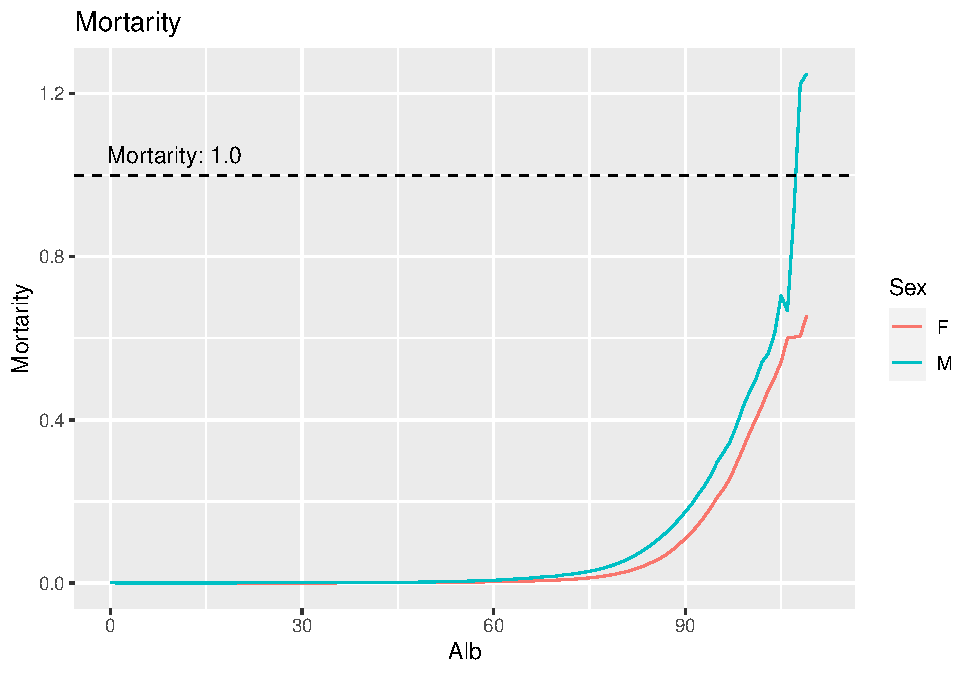
\includegraphics{python-medical-data_files/figure-latex/unnamed-chunk-10-1.pdf}

高齢部分が不自然だが、そういうものらしい。100才以上は使わない、として切り捨てる。

また、年次死亡率を月次死亡率に変換する。

年次死亡率を\(y\)、月次死亡率を\(x\)とすると、

\(y = 1 - (1-x)^{12}\)なので、\(x = 1 - (1-y)^{0.08...}\)になる。

\begin{Shaded}
\begin{Highlighting}[]
\NormalTok{dat }\OperatorTok
\StringTok{        }\KeywordTok{filter}\NormalTok{(Alb }\OperatorTok{<}\StringTok{ }\DecValTok{100}\NormalTok{)}

\NormalTok{dat }\OperatorTok\StringTok{ }
\StringTok{        }\KeywordTok{mutate}\NormalTok{(}\DataTypeTok{F =} \DecValTok{1} \OperatorTok{-}\StringTok{ }\NormalTok{(}\DecValTok{1}\OperatorTok{-}\NormalTok{F)}\OperatorTok{**}\NormalTok{(}\DecValTok{1}\OperatorTok{/}\DecValTok{12}\NormalTok{)) }\OperatorTok\StringTok{ }
\StringTok{        }\KeywordTok{mutate}\NormalTok{(}\DataTypeTok{M =} \DecValTok{1} \OperatorTok{-}\StringTok{ }\NormalTok{(}\DecValTok{1}\OperatorTok{-}\NormalTok{M)}\OperatorTok{**}\NormalTok{(}\DecValTok{1}\OperatorTok{/}\DecValTok{12}\NormalTok{)) }

\NormalTok{dat }\OperatorTok\StringTok{ }\KeywordTok{write.csv}\NormalTok{(}\StringTok{"./data/ipss_mortality.csv"}\NormalTok{, }\DataTypeTok{quote=}\NormalTok{F, }\DataTypeTok{row.names =}\NormalTok{ F)}
\NormalTok{dat }\OperatorTok\StringTok{ }\NormalTok{head}
\end{Highlighting}
\end{Shaded}

\begin{verbatim}
##   Alb            F            M
## 1   0 9.759403e-05 9.734377e-05
## 2   1 2.029393e-05 2.158590e-05
## 3   2 1.133404e-05 1.295926e-05
## 4   3 7.708660e-06 9.500496e-06
## 5   4 7.125279e-06 8.167034e-06
## 6   5 6.791920e-06 8.833763e-06
\end{verbatim}

おわり

\hypertarget{ux3053ux3053ux307eux3067ux3084ux3063ux305fux3053ux3068}{%
\subsection{ここまでやったこと}\label{ux3053ux3053ux307eux3067ux3084ux3063ux305fux3053ux3068}}

\begin{itemize}
\tightlist
\item
  公的統計の取得
\item
  出生率データの作成
\item
  死亡率データの作成
\end{itemize}

\hypertarget{ux3064ux304eux306bux3084ux308bux3053ux3068}{%
\subsection{つぎにやること}\label{ux3064ux304eux306bux3084ux308bux3053ux3068}}

擬似レセプトデータを作るために\ldots{}
- 出生のシミュレーション
- 死亡のシミュレーシ

\hypertarget{ux51faux751fux6b7bux4ea1ux306eux30b7ux30dfux30e5ux30ecux30fcux30b7ux30e7ux30f3}{%
\section{出生・死亡のシミュレーション}\label{ux51faux751fux6b7bux4ea1ux306eux30b7ux30dfux30e5ux30ecux30fcux30b7ux30e7ux30f3}}

出生と死亡をシミュレーションして、擬似健康保険組合データを作成する。

\hypertarget{ux51faux751fux306eux30b7ux30dfux30e5ux30ecux30fcux30b7ux30e7ux30f3}{%
\subsection{出生のシミュレーション}\label{ux51faux751fux306eux30b7ux30dfux30e5ux30ecux30fcux30b7ux30e7ux30f3}}

\hypertarget{ux6b7bux4ea1ux306eux30b7ux30dfux30e5ux30ecux30fcux30b7ux30e7ux30f3}{%
\subsection{死亡のシミュレーション}\label{ux6b7bux4ea1ux306eux30b7ux30dfux30e5ux30ecux30fcux30b7ux30e7ux30f3}}

\hypertarget{ux307eux3068ux3081}{%
\subsection{まとめ}\label{ux307eux3068ux3081}}

  \bibliography{book.bib}

\end{document}
